\section{Ein System zur Klassifizierung einer Webseite}
    \label{section:conceptClassification}
    Der Spezifikation eines Klassifizierungsmodells folgt die Durchführung einer Klassifizierung,
    worüber dieses Kapitel einen allgemeinen Überblick verschafft.

    \subsection{Datenquelle}
        \label{section:conceptClassificationDataSource}
        Die erste zu klärende Frage ist, welche Repräsentation einer Webseite
        das \gls{wccs} zur Klassifizierung verwendet und woher es diese bezieht.
        Für den Fall der {\fernUni} bietet {\wordpress} zwei Schnittstellen,
        um Informationen über Beiträge und Seiten abzufragen:

        \begin{enumerate}
            \item Die Datenbanktabelle \texttt{wp\_posts} \cite[Kapitel "`Database Description"']{wordpress:codex} und
            \item einen RESTful Webservice \cite[Kapitel "`REST API Handbook"']{wordpress:codex}.
        \end{enumerate}

        Beide Quellen stellen das \gls{wccs} vor Herausforderungen.
        Die Inhalte der Datenbank speichern neben \gls{html} die Shortcodes
        von Plugins.
        Diese müssen ausgewertet werden, damit das \gls{wccs} die erzeugten Inhalte
        erfassen kann.
        Der RESTful Webservice übernimmt diese Aufgabe und übermittelt
        eine reine \gls{html}-Repräsentation des angeforderten Beitrages,
        was ein Argument für seine Verwendung ist.
        Allerdings ist auch über diesen Dienst nur das spezielle \gls{html}-Fragment eines
        Posts oder einer Page zugänglich.
        Inhalte, die über Templates in die vollständige Webseite gelangen,
        können über beide Schnittstellen nicht bezogen werden.
        Im Fall der Mitarbeiterseite\footnote{Ein Bildschirmaufnahme der Webseite
        ist in Abbildung \ref{image:findingTeachersModelOverview} in Kapitel
        \ref{section:findingsTeachersConceptualModel} zu sehen.}
        der Fakultät \gls{ksw}
        kann also das \gls{html}-Fragment mit der Überschrift, der Einleitung
        und der Mitarbeiterliste bezogen werden.
        Der Kopfbereich, der außerhalb des Posts der Seite definiert wird,
        hingegen nicht.
        Ob dies ein gravierendes Manko ist, hängt unter anderem davon ab,
        ob solche allgemeinen Bereiche relevant für eine Klassifizierung sind.
        Ein Nachteil ist allerdings, dass externe Systeme über diese Schnittstellen
        nur schwer ermitteln können, wo die Inhalte eines Beitrages auf der vollständigen Webseite genau positioniert sind.
        Das erschwert dem \gls{wccs} die Visualisierung einer
        Klassifikation auf der Webseite\footnote{vgl. Kapitel \ref{section:conceptVisualization}}.       
        Ein weiterer zu beachtender Aspekt ist, dass diese Quellen {\wordpress}-spezifisch sind,
        wodurch eine starke Bindung zu diesem \gls{cms} entsteht
        und das \gls{wccs} weniger allgemein einsatzbar wird.

        Eine Alternative, um diese Probleme zu lösen,
        ist die Nutzung der \gls{html}-Repräsentation einer Webseite,
        die über ihre \gls{url} bezogen wird.
        Diese verwendet eine standardisierte Sprache (\gls{html}) und enthält
        alle Bereiche und Inhalte der Seite.
        Es können also auch global definierte Inhalte,
        wie der Kopfbereich, leicht einer Klassifizierung unterzogen werden.
        Gleichzeitig macht es das \gls{wccs} vollkommen unabhängig vom verwendeten \gls{cms},
        da es im konkreten Fall z. B. nichts über Shortcodes und deren Auswertung wissen muss.
        Diese Aufgabe übernimmt {\wordpress}.

    \subsection{Ablauf einer Klassifizierung}
        \label{section:solutionConceptClassificationAlg}
        Der allgemeine Ablauf der Klassifizierung lässt sich leicht und in wenigen Sätzen beschreiben.
        Zur Durchführung einer Klassifizierung erwartet das \gls{wccs} die \gls{url} einer Webseite,
        da sie dessen \gls{html}-Repräsentation als Datenquelle verwendet.
        Basierend auf dem bereitgestellten Klassifizierungsmodell
        bestimmt das System zunächst die Klasse der Seite,
        indem es die Selektoren der bekannten Seitenklassen gegen sie prüft.
        Anschließend ermittelt das \gls{wccs} die Features dieser Klasse auf der vorliegenden Webseite,
        indem die Selektoren der Features auf der Seite angewandt werden.
        Für jedes {\contentFeature} sucht es außerdem rekursiv nach allen {\childFeature}s.
        Ist dieser Prozess beendet, werden die gesammelten Informationen in Form einer Klassifikation
        dauerhaft persistiert.

    \subsection{Selektoren}
        \label{section:conceptSupportedSelectors}
        Das \gls{wccs} unterstützt drei Arten von Selektoren:

        \begin{enumerate}
            \item CSS,
            \item XPath und
            \item reguläre Ausdrücke auf \glspl{url}.
        \end{enumerate}

        \paragraph{Der \cssSelector}
        Zur Bestimmung beider Arten von Features unterstützt das \gls{wccs} zunächst
        die Auswertung von {\cssSelector}en, die durch das \gls{w3c} standardisiert
        sind\footnote{vgl. Kapitel \ref{section:problemAnalysisWebpagesInTheWWWSeparationOfConcerns}}.
        Durch einen einzelnen {\cssSelector} können potenziell viele Elemente im \gls{html}-Dokument
        erfasst werden, wodurch {\collectionFeature}s realisierbar sind.
        Jedes selektierte Element stellt dabei genau ein Feature dar.
        Das \gls{wccs} folgt bei der Auswertung eines {\cssSelector}s der Logik des \glspl{w3c}.
        Das bedeutet, dass der Selektor auf das gesamte Dokument angewandt wird,
        aber nur Elemente innerhalb des Elementes des {\parentFeature}s -- dem Kontextelement --
        im Ergebnis enthalten sind \cite{w3c:selectorsAPI}.
        Bei den Features der Seitenklasse wird hingegen die gesamte Seite als Kontext verwendet,
        weshalb keine Filterung der Ergebnisse des Selektors stattfindet.
        Durch dieses Vorgehen können sich wiederholende Strukturen auf einer Webseite
        korrekt durch Elemente eines {\collectionFeature}s dargestellt werden.
        Zur Veranschaulichung dient der Ausschnitt eines \gls{html}-Dokumentes
        in Listing \ref{listing:conceptCssSelectorExample}.

        \begin{lstlisting}[
            label=listing:conceptCssSelectorExample,
            caption=Ein Beispiel einer sich wiederholenden Struktur in einem \acrshort{html}-Dokument,
            style=html]
<article>
    <h3>Article 1 Heading<h3>
</article>
<article>
    <h3>Article 2 Heading<h3>
</article>
<article>
    <h3>Article 3 Heading<h3>
</article>
        \end{lstlisting}

        Dieses Beispiel enthält mehrere Artikel, die jeweils eine Überschrift besitzen.
        Die Artikel können über den Namen ihres Elementes angesprochen werden.
        Das heißt der {\cssSelector} des {\collectionFeature}s ist \texttt{article}.
        Die Klasse dieses Features enthält ihrerseits ein Feature für die Überschrift,
        welches den Selector \texttt{h3} verwendet.
        Dieser Selektor wird im Kontext des Elementes seines {\parentFeature}s ausgeführt,
        das heißt im Kontext eines \texttt{article}-Elementes.
        Dadurch erfasst er immer nur das \texttt{h3} innerhalb des \texttt{article}s,
        wodurch gewährleistet ist, dass ausschließlich die Überschrift des aktuellen Artikels erfasst wird.
        Das \gls{wccs} kann jedem Artikel also die korrekte Überschrift zuordnen.

        \paragraph{Der \xpathSelector}
        Eine weitere Möglichkeit sowohl {\contentFeature}s als auch {\referenceFeature}s
        zu erfassen, ist die Nutzung von XPath-Ausdrücken,
        die dazu auf dem \gls{html}-Dokument angewandt
        werden\footnote{Kapitel \ref{section:solutionDetailsClassificationServiceClassification}
        beschreibt, wie dies möglich ist, obwohl \gls{html}-Dokumente oftmals kein
        valides XML verwenden.}.
        Mit XPath können analog zu CSS \gls{html}-Elemente der Seite erfasst werden
        \cite{w3c:xpath},
        weshalb auch die Logik des \glspl{wccs} bei der Auswertung eines {\xpathSelector}s der gleichen Idee folgt.
        Das heißt, dass auch hier das Element des {\parentFeature}s
        als Kontextelement verwendet wird.
        Das Ergebnis eines XPath-Ausdruckes kann aber auch reiner Text sein
        \cite{w3c:xpath},
        der vom \gls{wccs} je nach Art des Features als Inhalt oder als Ziel einer
        Referenz gewertet wird.
        Im Vergleich zu CSS ist XPath in einigen Belangen mächtiger.
        Zum Beispiel erlaubt es die Erfassung des aktuellen Kontextelementes
        oder dessen Geschwister \cite{w3c:xpath}.
        Die garantierte Relativität eines {\cssSelector}s ist durch
        einen {\xpathSelector} also nicht immer gegeben,
        wodurch der Verfasser eines Klassifizierungsmodells mehr Möglichkeiten,
        aber auch mehr Verantwortung erhält.

        \paragraph{Der \gls{url}-Pattern-Selektor}
        Das \gls{wccs} bietet die Möglichkeit reguläre Ausdrücke auf \glspl{url} anzuwenden,
        was sich zur Klassifizierung einer Webseite als Ganzes und von {\referenceFeature}s eignet.
        Im Falle von Webseiten wird der Ausdruck lediglich auf die \gls{url} angewandt
        und eine Übereinstimmung als Erfüllung des Selektors interpretiert.       
        Zur Klassifizierung von Referenzen wird der Selektor auf die \glspl{url} aller Knoten
        innerhalb des Kontextelementes angewandt, die eine {\resource} referenzieren.
        Jedes Element, welches eine Übereinstimmung mit dem regulären Ausdruck besitzt,
        wird vom \gls{wccs} als {\referenceFeature} klassifiziert.
        Mit dem {\urlSelector} sind demnach auch {\collectionFeature}s realisierbar.

        % TODO: Hier oder bei den Ergebnissen? Dieser Selektor ist sinnvoll, um zum Beispiel externe Links anders als interne zu klassifizieren.

    \subsection{Datenmodell einer Klassifikation}
        \label{section:conceptPageDataModel}
        Die vom \gls{wccs} erzeugten Klassifikationen folgen dem
        in Abbildung \ref{image:conceptPageDataModel} dargestellten Datenmodell.

        \begin{figure}[htb]
            \centering
            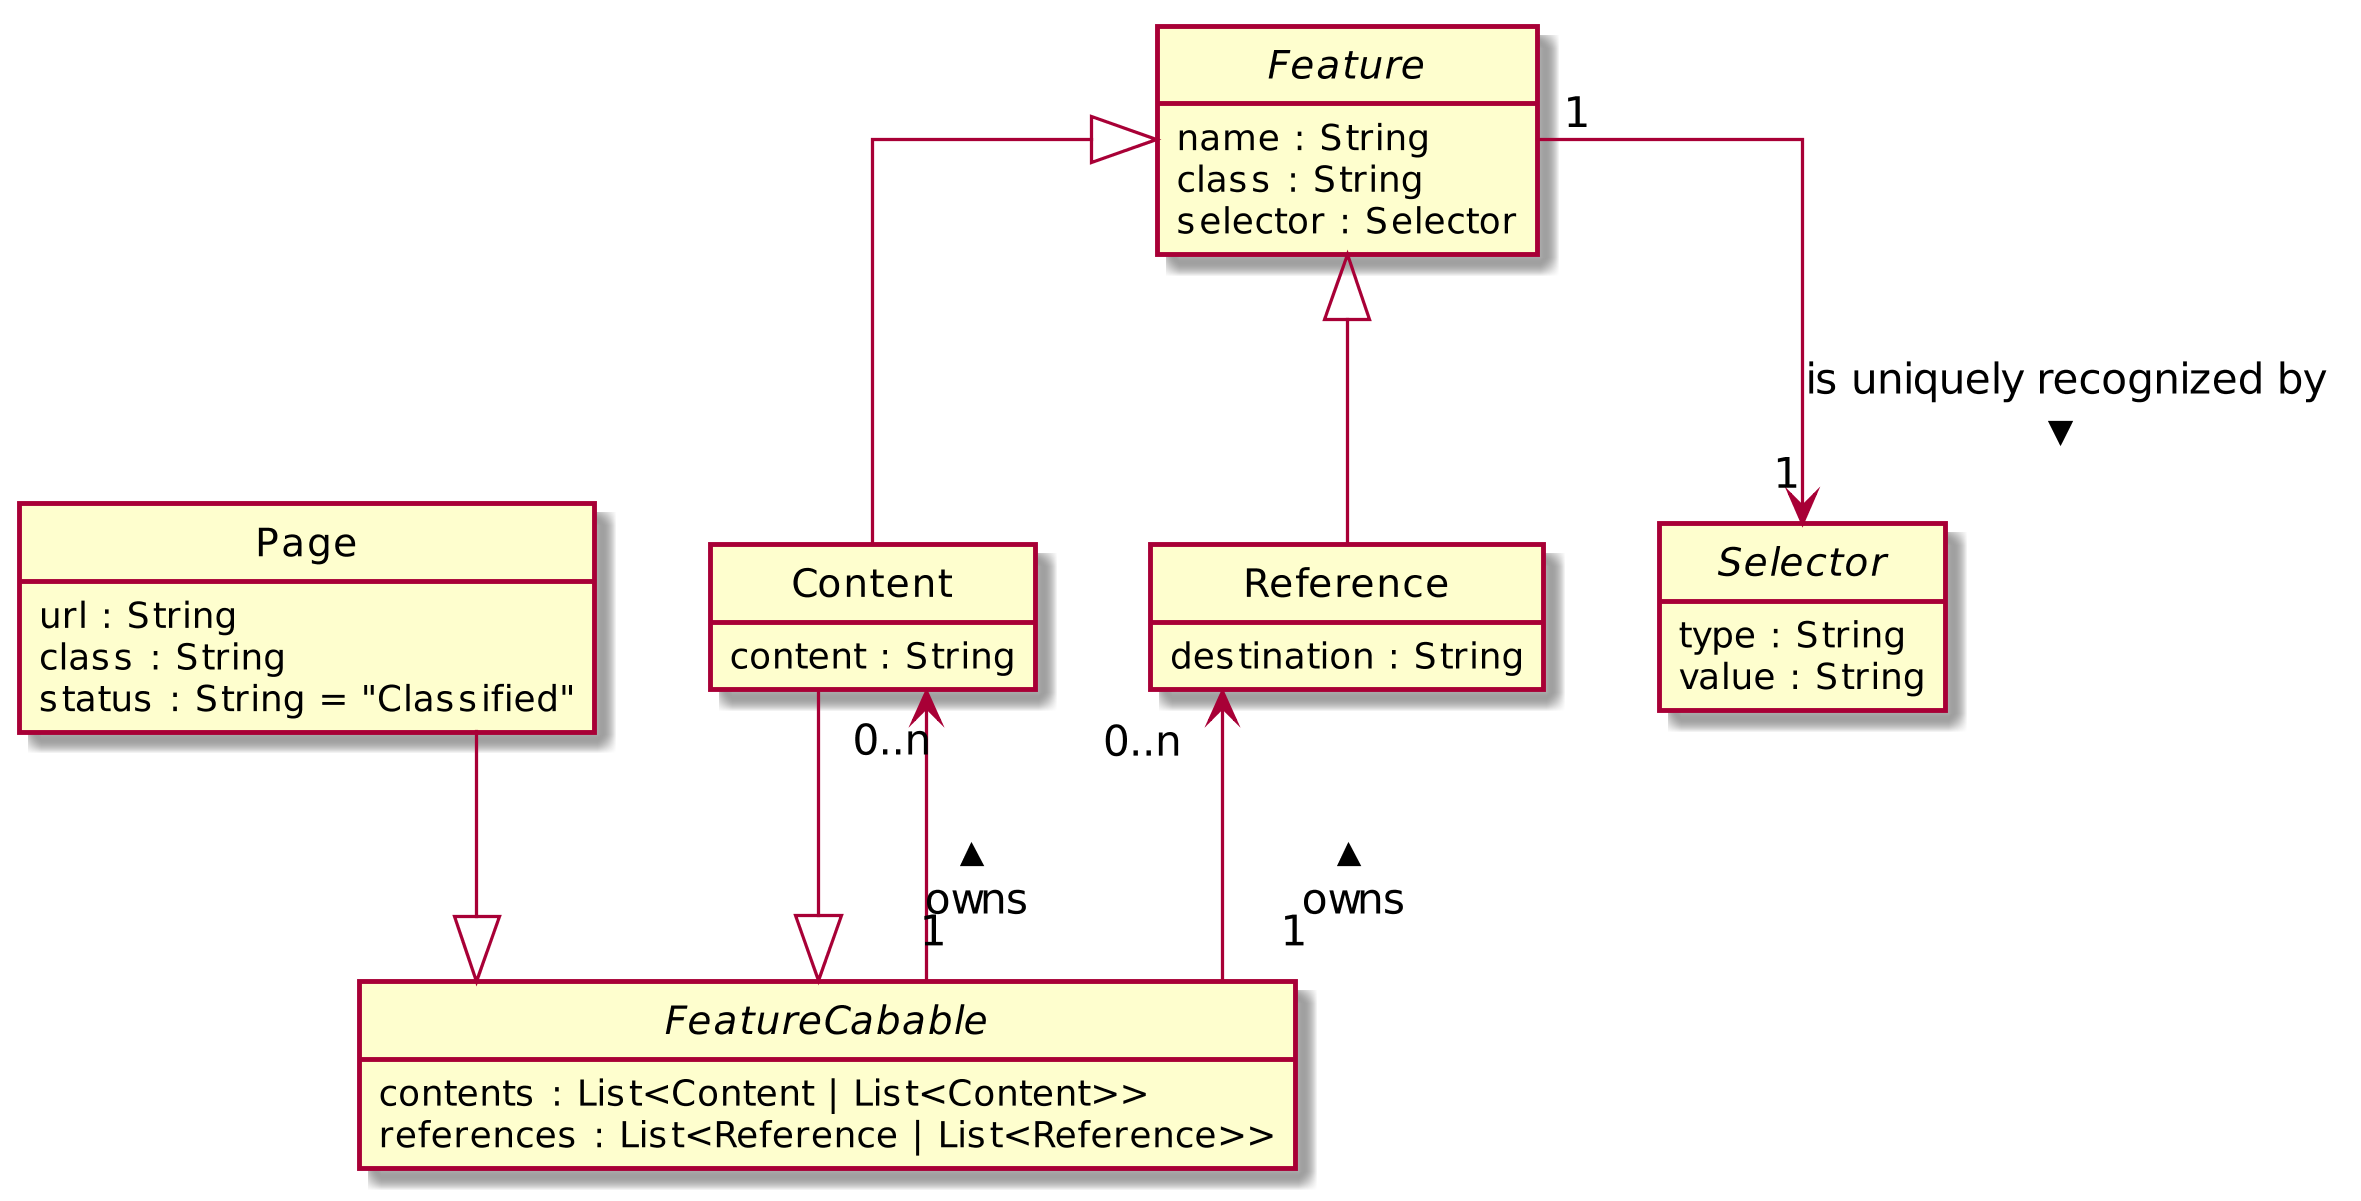
\includegraphics[scale=\imageScalingFactor]{../resources/concept/page.png}
            \caption{Das Datenmodell einer Klassifikation}
            \label{image:conceptPageDataModel}
        \end{figure}

        Eine Klassifikation beschreibt zunächst die betroffene Webseite,
        indem sie ihre \gls{url}, Klasse und Status speichert,
        der nach einer Klassifizierung generelle den Wert "`Classified"' hat.       
        Des Weiteren enthält sie in zwei getrennten Listen die {\contentFeature}s
        und {\referenceFeature}s der Seite, was in Abbildung \ref{image:conceptPageDataModel}
        durch die Vererbungshierarchie zwischen \texttt{Page} und \texttt{FeatureCapable}
        dargestellt wird.
        Elemente dieser Listen können neben \texttt{Content}- und \texttt{Reference}-Objekten
        auch Listen solcher Objekte sein,
        wodurch zwischen {\scalarFeature}s und {\collectionFeature}s unterschieden wird.
        {\contentFeature}s speichern ihren textuellen Inhalt,
        {\referenceFeature}s wiederum ihre \gls{url}.
        Dadurch stellt eine Klassifikation eine Momentaufnahme der relevanten Inhalte
        einer Webseite dar und spiegelt Änderungen an der Seite nicht
        automatisch wider.
        Außerdem erlaubt es Drittsystemen die konkreten Inhalte und Referenzen
        direkt zu nutzen, ohne sie von der Webseite erneut zu beziehen.
        Neben diesen individuellen Informationen enthält jedes Feature
        seinen Namen, seine Klasse und einen Selektor.
        Dabei handelt es sich nicht um den Selektor des Klassifizierungsmodells,
        mit dem das Feature erfasst wurde,
        sondern um einen Ausdruck, der das zugehörige Element im \gls{html}-Dokument eindeutig identifiziert.
        Auch jeder Eintrag eines {\collectionFeature}s besitzt demnach einen anderen Selektor.
        Dieser Selektor ermöglicht die spätere Visualisierung einer
        Klassifikation\footnote{vgl. Kapitel \ref{section:conceptVisualization} und
        \ref{section:solutionDetailsAnnotationServiceMapping}}
        und bietet Drittsystemen eine Möglichkeit zu prüfen,
        ob der klassifizierte Inhalt immer noch aktuell ist.
        Das Format des Selektors wird an dieser Stelle nicht weiter spezifiziert,
        da mehrere Methoden denkbar sind, um eine eindeutige Identifizierung eines Features
        umzusetzen\footnote{vgl. Kapitel \ref{section:solutionDetailsClassificationServiceClassification}} .
